\documentclass[tikz]{standalone}
\usepackage[utf8]{inputenc}
\usepackage{tikz}
\usepackage{flowchart}
\usetikzlibrary{shapes.geometric, arrows}
\tikzstyle{arrow} = [ very thick,->,>=stealth]
\begin{document}
    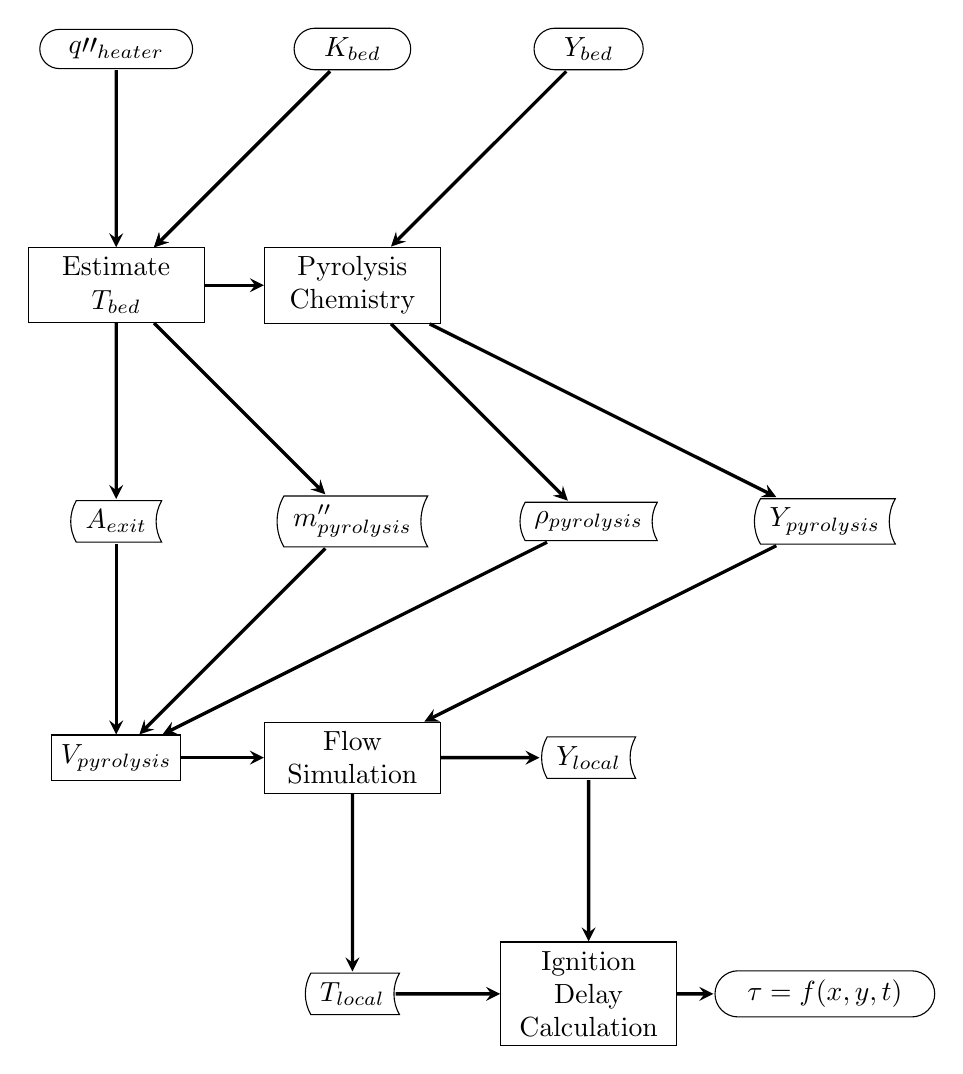
\begin{tikzpicture}[node distance=3cm and 2cm]
    
        \node (tbed) [draw, process, text width=2cm, text centered ] {Estimate $T_{bed}$};
        \node (qprime) [draw, terminal, above of=tbed] {$q\prime\prime_{heater}$};
        \node (kbed) [draw, terminal, right of=qprime] {$K_{bed}$};
        \node (ybed) [draw, terminal, right of=kbed] {$Y_{bed}$};
        \node (pchem) [draw, process, right of=tbed, text width=2cm, text centered] {Pyrolysis Chemistry};
        \node (aexit) [draw, storage, below of=tbed] {$A_{exit}$};

        \node (mflux) [draw, storage, right of=aexit] {$m^{\prime \prime}_{pyrolysis}$};
        \node (rhogas) [draw, storage, right of=mflux] {$\rho_{pyrolysis}$};
        \node (yprod) [draw, storage, right of=rhogas] {$Y_{pyrolysis}$};


        \node (vgas) [draw, process, below of=aexit] {$V_{pyrolysis}$};
        \node (flowsim) [draw, process, right of = vgas, text width=2cm, text centered] {Flow Simulation};
        \node (ygas) [draw, storage, right of=flowsim] {$Y_{local}$};
        \node (tgas) [draw, storage, below of=flowsim] {$T_{local}$};
        \node (delay) [draw, process,  right of=tgas, text width=2cm, text centered] {Ignition Delay Calculation};

        \node (tau) [draw, terminal, right of=delay] {$\tau = f(x, y, t)$};
        
        \draw [arrow] (kbed) -- (tbed);
        \draw [arrow] (qprime) -- (tbed);
        \draw [arrow] (tbed) -- (pchem);
        \draw [arrow] (tbed) -- (mflux);
        \draw [arrow] (tbed) -- (aexit);
        \draw [arrow] (kbed) -- (tbed);
        \draw [arrow] (ybed) -- (pchem);
        \draw [arrow] (pchem) -- (rhogas);
        \draw [arrow] (pchem) -- (yprod);
        \draw [arrow] (rhogas) -- (vgas);
        \draw [arrow] (mflux) -- (vgas);
        \draw [arrow] (aexit) -- (vgas);
        \draw [arrow] (vgas) -- (flowsim);
        \draw [arrow] (yprod) -- (flowsim);
        \draw [arrow] (flowsim) -- (tgas);
        \draw [arrow] (flowsim) -- (ygas);
        \draw [arrow] (tgas) -- (delay);
        \draw [arrow] (ygas) -- (delay);
        \draw [arrow] (delay) -- (tau);
    \end{tikzpicture}
\end{document}